%!TEX root = ../thesis.tex
\chapter{Design \& Implementation}

	Development of a graphical user interface for libmapper creates a unique challenge. Obviously such an interface is a practical tool, and should function as such, yet it also must work in concert with DMIs which are inherently designed for abstract and creative use. For the purposes of this project, the assumed solution to this innate paradox is to provide the user with multiple independent modes of control.  This assumption was made based on experiences with prior user interfaces for libmapper (vizmapper, max mapperGUI): for each interface users reported excellent functionality for certain use cases, and poor functionality for others. Libmapper itself is an extremely flexible API that makes few assumptions as to the network of devices and signals, nor how they are being mapped. It is fitting that a GUI for libmapper would be equally as flexible. In lieu of a single perfect solution for network visualization an interactivity, providing users with various independent solutions provided a good compromise.
	

\section{Development of a Flexible Interface (Development Background)}
	
Prior GUIs for libmapper have been successfully used for some time, but all fail for one reason: they cannot accomidate all possible use-cases of libmapper. 
	%Needs to be adaptable, show any metadata

\subsection{List view}
\label{sec:list_view}
\subsection{Grid view}
\subsection{Hive plot}
\subsection{Cluster view (vizmapper)}

\section{Control Features}
\subsection{Creating Connections/Links}
\subsection{Modifying Signals}

\section{The Model-View-Controller}

	Because a modular design is desired, the Model-View-Controller (MVC) metaphor for structuring software applications as described in [KrasnerPope88] was used as a general framework for structuring the application. In fact, the whole scale swapping in and out of independent visual modes can be thought of as a quintessential implementation of MVC. 
	
\subsection{The Model}

	The model consists of an abstract copy of the network, residing on the local machine. Independent views can consult this data, but cannot directly modify it.

\subsection{Controller-View Pairs}

\section{Graphical Design}
	wiggly arrows
\subsection{Typography}

\begin{figure}[ht]
\centering
	\scalebox{0.4}{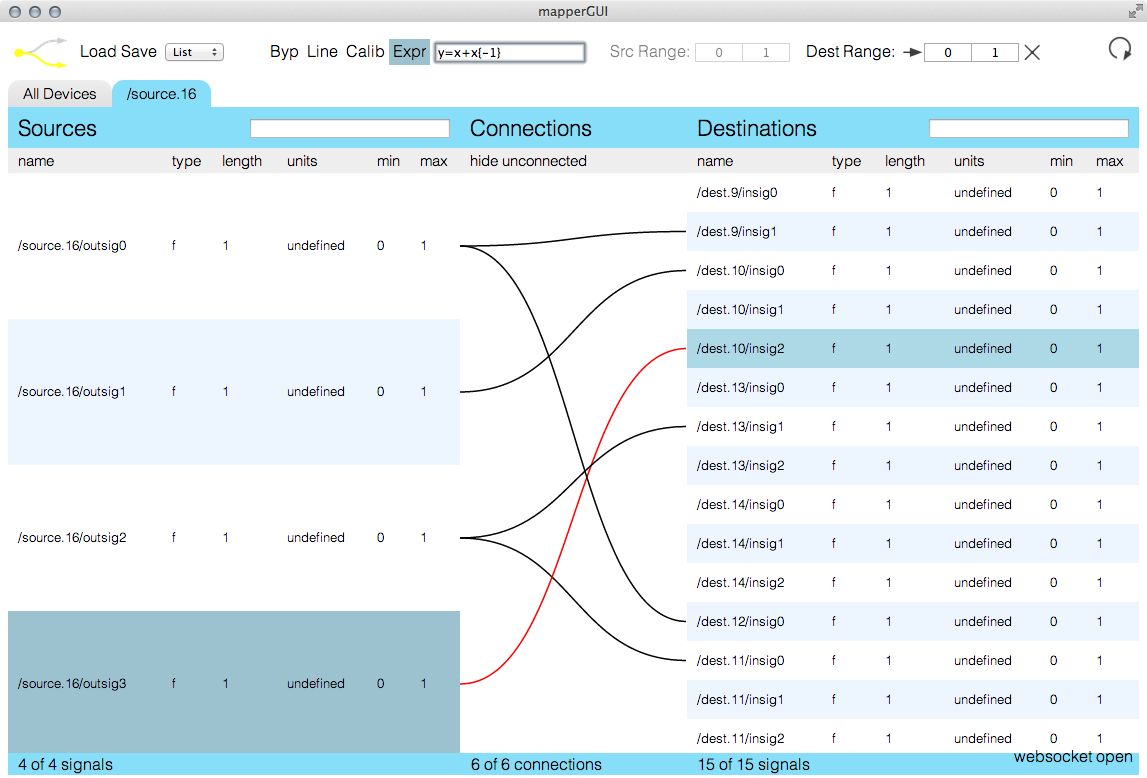
\includegraphics{figures/final_list}}
\caption{The list view after redesign}
\label{fig:final_list}
\end{figure}

\begin{figure}[ht]
\centering
	\scalebox{0.4}{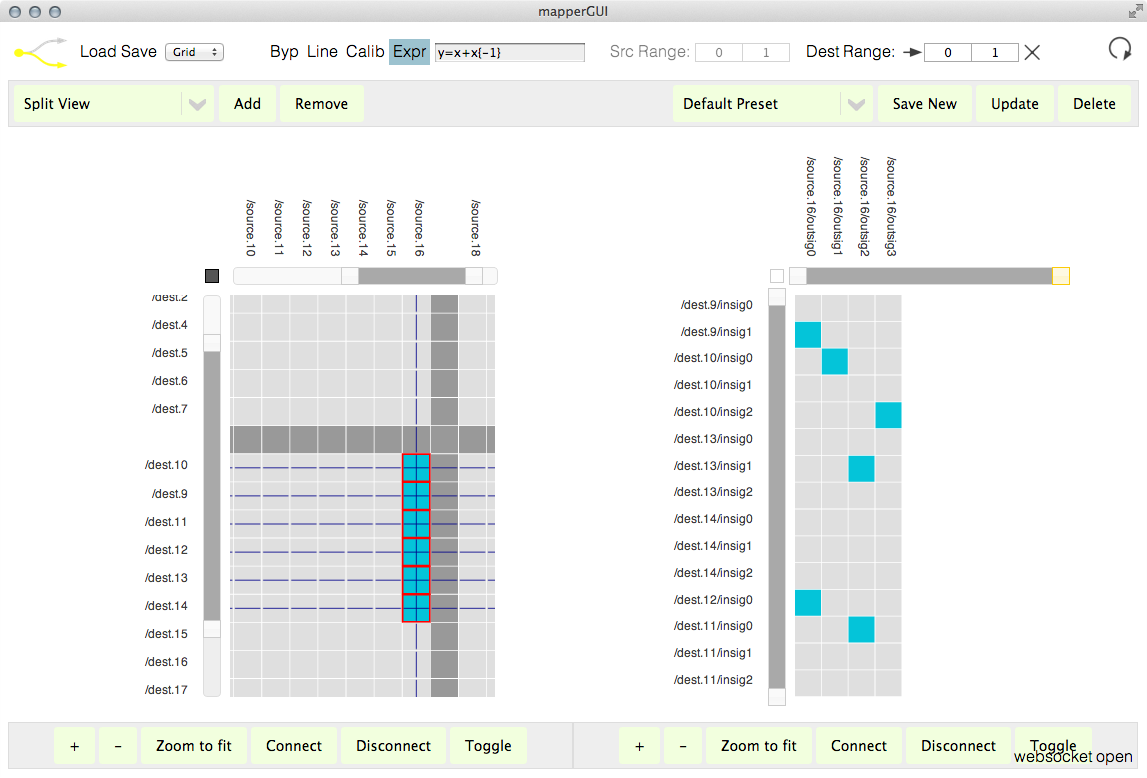
\includegraphics{figures/grid}}
\caption{The grid view}
\label{fig:grid}
\end{figure}

\begin{figure}[ht]
\centering
	\scalebox{0.4}{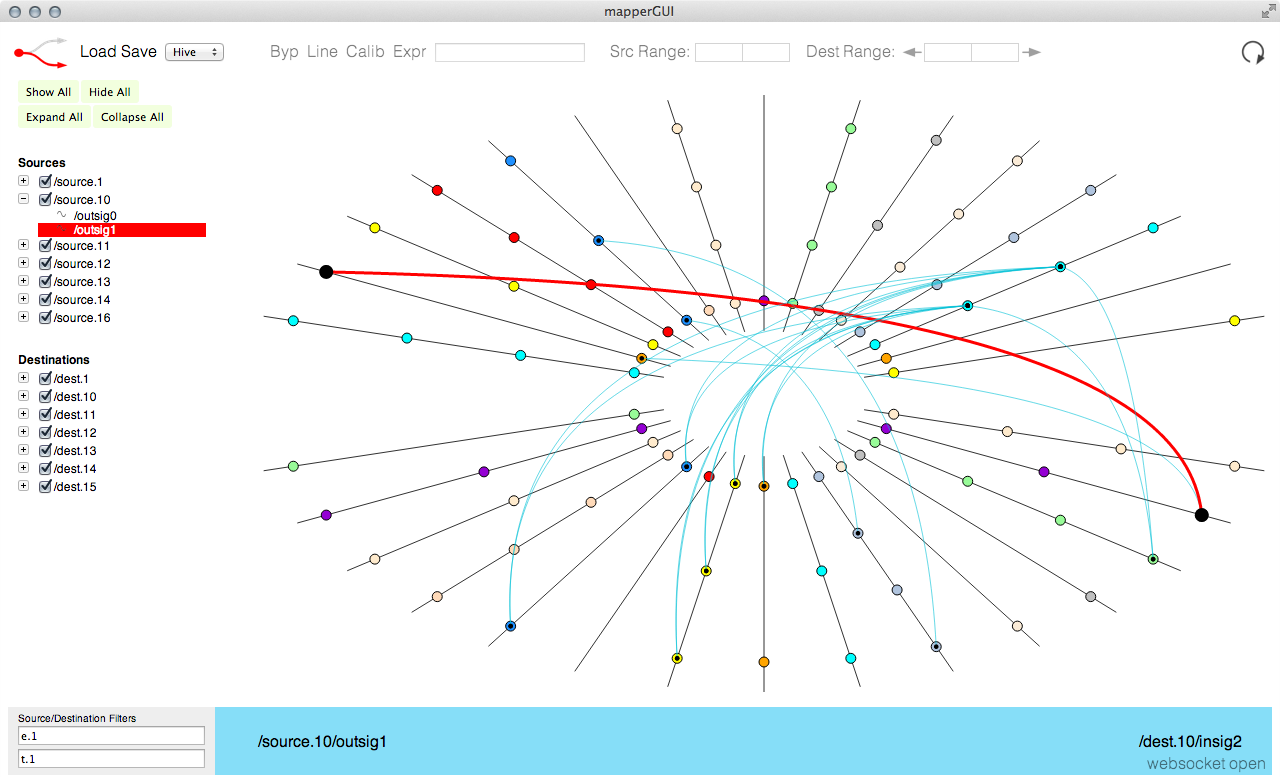
\includegraphics{figures/hive}}
\caption{The hive view}
\label{fig:hive}
\end{figure}

	
\section{User Centric Design}
	use cases

\section{Robustness and Responsiveness}
	speed tests